\documentclass[11pt,a4paper]{article}

% -----------------------------------------------------------------------------
% Working draft v1.1
% Article language: British English
% Title constraint: no colon, not more than 12 words
% -----------------------------------------------------------------------------

\usepackage[margin=2.3cm]{geometry}
\usepackage[T1]{fontenc}
\usepackage[utf8]{inputenc}
\usepackage{lmodern}
\usepackage{microtype}
\usepackage{setspace}
\usepackage{booktabs}
\usepackage{tabularx}
\usepackage{longtable}
\usepackage{array}
\usepackage{enumitem}
\usepackage{graphicx}
\usepackage{xcolor}
\usepackage{tikz}
\usepackage{pgfplots}
\usepackage{xurl}
\usepackage{hyperref}
\usepackage{cleveref}
\usepackage[numbers,sort&compress]{natbib}
\usepackage{caption}
\usepackage{subcaption}
\usepackage{float}

\pgfplotsset{compat=1.18}
\usetikzlibrary{arrows.meta,positioning,fit,shapes.geometric,shapes.misc,calc,matrix,backgrounds,decorations.pathreplacing}


% Unified diagram styles for article figures
\tikzset{
  dbox/.style={draw, rounded corners=2pt, thick, align=center, text width=2.9cm, minimum height=1.0cm, inner sep=3pt, fill=blue!5, font=\sffamily\small},
  dboxwide/.style={draw, rounded corners=2pt, thick, align=center, text width=3.2cm, minimum height=1.0cm, inner sep=3pt, fill=blue!5, font=\sffamily\small},
  dphase/.style={draw, rounded corners=2pt, thick, align=center, text width=2.7cm, minimum height=1.0cm, inner sep=3pt, fill=gray!10, font=\sffamily\small},
  dobs/.style={draw, rounded corners=2pt, thick, align=center, text width=3.0cm, minimum height=1.0cm, inner sep=3pt, fill=green!8, font=\sffamily\small},
  dstore/.style={draw, cylinder, shape border rotate=90, aspect=0.25, align=center, minimum width=2.0cm, minimum height=1.0cm, fill=yellow!12, font=\sffamily\small},
  dnote/.style={font=\sffamily\scriptsize, align=center, fill=white, inner sep=1.5pt},
  darrow/.style={-Latex, thick},
  dfeedback/.style={-Latex, thick, dashed},
  dframe/.style={draw, dashed, rounded corners, inner sep=4mm},
  dlayer/.style={draw, rounded corners=2pt, thick, align=center, minimum width=10.6cm, minimum height=0.82cm, inner sep=3pt, font=\sffamily\small},
  ddone/.style={draw, rounded corners=2pt, thick, align=center, text width=3.0cm, minimum height=0.95cm, inner sep=3pt, fill=green!10, font=\sffamily\small},
  dplanned/.style={draw, rounded corners=2pt, thick, align=center, text width=3.0cm, minimum height=0.95cm, inner sep=3pt, fill=orange!10, font=\sffamily\small}
}

\hypersetup{
  colorlinks=true,
  linkcolor=blue!60!black,
  citecolor=blue!60!black,
  urlcolor=blue!60!black,
  pdftitle={From Synthetic Benchmarks to Feedback-Controlled Testbeds: Observability and Workload Management in a Containerised Solana Localnet},
  pdfauthor={Author Name}
}

\setstretch{1.08}
\setlist[itemize]{topsep=3pt,itemsep=2pt,parsep=0pt}
\setlist[enumerate]{topsep=3pt,itemsep=2pt,parsep=0pt}

\newcolumntype{Y}{>{\raggedright\arraybackslash}X}
\newcolumntype{L}[1]{>{\raggedright\arraybackslash}p{#1}}
\newcommand{\todo}[1]{\textcolor{red!70!black}{[TODO: #1]}}
\newcommand{\artifact}{artefact}
\newcommand{\artifacts}{artefacts}

\title{From Synthetic Benchmarks to Feedback-Controlled Testbeds: Observability and Workload Management in a Containerised Solana Localnet}
\author{Author Name\\
\small Affiliation\\
\small \texttt{email@example.org}}
\date{Working draft v1.1 empirical pilot update}

\begin{document}
\maketitle

\begin{abstract}
Synthetic benchmarks have historically provided simplified and repeatable workloads for comparing computing systems, but contemporary distributed systems require a broader evaluation model. They are telemetry-rich, resource-constrained, dynamically operated, and increasingly shaped by feedback mechanisms. This paper argues that synthetic benchmarking is therefore evolving from open-loop performance measurement towards reproducible experimental testbeds in which workload generation, observability, dataset production, and future control interfaces are designed together. The argument is developed as a methodological contribution and illustrated through a containerised private Solana network consisting of a validator, wallet and workload components, Yellowstone/Geyser-based observability, monitoring services, and Prometheus-compatible metrics. The paper also reports a preliminary single-host empirical pilot consisting of three baseline runs, two low transaction-load runs, and two medium transaction-load runs. The pilot is not presented as a general Solana performance study. Instead, it validates the article's measurement discipline: the data-collection pipeline preserves hostname-aware metadata, validator health samples, RPC-level slot and transaction counters, and workload-side transaction evidence. The results show stable health across all included runs and a clear increase in transaction-count deltas under controlled workload profiles. The resulting case study positions the Solana testbed as a reproducible research infrastructure for studying high-performance blockchain behaviour under controlled synthetic workloads and for preparing later feedback-control experiments with rule-based controllers, classical baselines, model-predictive approaches, and multi-agent reinforcement learning.
\end{abstract}

\noindent\textbf{Keywords:} synthetic benchmark; distributed systems; Solana; testbed; observability; Geyser; Yellowstone gRPC; Prometheus; feedback control; multi-agent reinforcement learning; reproducible research.

\section{Introduction}
\label{sec:introduction}

Performance evaluation has long been a central activity in computer systems research. Synthetic benchmarks made it possible to compare machines, compilers, operating systems, databases, and networked services using workloads that were deliberately simplified, repeatable, and portable. Classical examples such as Whetstone and Dhrystone were designed to capture representative computational behaviour using compact programs rather than complete applications. Later benchmark families expanded the idea towards application suites, database transaction processing, decision support workloads, graph analytics, machine learning, and energy-aware evaluation \cite{weicker1984dhrystone,mdpi2025benchmarking}.

This historical trajectory is often described as a progression from simple synthetic programs towards richer, domain-specific suites. That description is accurate but incomplete. The most important transition in modern distributed systems is not merely that benchmarks have become larger or more realistic. Rather, the benchmark is increasingly becoming an experimental environment. It contains a workload generator, an observability layer, a configuration interface, a dataset pipeline, and, in advanced cases, a feedback controller. This change reflects the operational reality of distributed systems: throughput and latency remain important, but they no longer exhaust the research problem. A modern benchmark must also help answer how a system behaves under perturbation, how it exposes internal state, how reproducible its measurements are, and whether measured behaviour can be used to make safe adaptive decisions.

High-performance blockchain networks provide a useful case for this shift. They combine distributed consensus, transaction processing, resource contention, event streams, RPC interfaces, and strong requirements for reproducibility. Solana is a particularly relevant example because it is designed for high-throughput operation and exposes validator-side streaming mechanisms such as Geyser plugins. The Agave validator documentation describes Geyser as a plugin mechanism through which validator information about accounts, slots, blocks, and transactions can be transmitted to external systems, partly addressing the risk that validators under heavy RPC loads fall behind the network \cite{anza2026geyser}. Yellowstone gRPC builds on this Geyser interface by providing a gRPC-based streaming path for slots, blocks, transactions, and account updates \cite{rpcpool2026yellowstone}.

This paper uses a containerised private Solana local network as a concrete case study. The associated public repository describes a containerised local Solana testbed for dataset generation and latency/performance research, and frames it as a migration from a virtual-machine-based local testbed towards a reproducible Podman/Docker Compose architecture \cite{okhoshaba2026repo}. The repository also references persistent Zenodo records for a Solana v1.18.25 local testbed and for a Yellowstone/Geyser observability extension \cite{khoshaba2026containerising,khoshaba2026yellowstone}.

The central thesis is as follows:

\begin{quote}
Synthetic benchmarking in distributed systems is evolving from the measurement of isolated performance limits towards the construction of reproducible, observable, and eventually controllable experimental environments.
\end{quote}

Accordingly, the Solana example is not treated as a narrow engineering demonstration. It is used to articulate a more general methodological pattern: a benchmark becomes scientifically stronger when it is designed as a closed research loop connecting workload, observation, artefact production, and control.

\subsection{Research questions}
\label{subsec:research-questions}

The article is organised around four research questions. They are deliberately methodological rather than benchmark-result questions, because the current paper is concerned with the design of an experimental infrastructure and the evidence required for future empirical claims.

\begin{table}[H]
\centering
\caption{Research questions guiding the article}
\label{tab:research-questions}
\begin{tabularx}{\textwidth}{L{1.2cm}Y Y}
\toprule
\textbf{ID} & \textbf{Research question} & \textbf{Expected contribution} \\
\midrule
RQ1 & How can synthetic benchmarking in distributed systems be reframed from maximum-performance measurement towards observable and reproducible experimentation? & A conceptual model that links workload generation, orchestration, observability, datasets, and control interfaces. \\
RQ2 & What design requirements must a benchmark satisfy before it can support feedback-oriented or adaptive control experiments? & A requirement set covering reproducibility, workload parametrisation, observability, metadata, perturbations, and baseline comparability. \\
RQ3 & How can a containerised Solana localnet serve as a concrete case study for a control-oriented distributed-systems testbed? & An architecture mapping Solana validator, Yellowstone/Geyser, monitor services, Prometheus metrics, and datasets to research roles. \\
RQ4 & What evidence is still required before stronger claims about Solana performance, observability overhead, or learning-based control can be made? & An implementation-boundary and evidence-plan framework that separates current artefacts from planned empirical validation. \\
\bottomrule
\end{tabularx}
\end{table}

\subsection{Contributions}
\label{subsec:contributions}

The paper makes seven contributions.

\begin{enumerate}
  \item It reframes synthetic benchmarking as a progression from performance measurement to reproducible, observable, and control-ready experimental infrastructure.
  \item It clarifies the distinction between a synthetic benchmark, workload generator, testbed, observability layer, dataset, and controller.
  \item It positions the argument against related work on benchmark evolution, workload-driven systems, self-management, observability, and learning-based resource allocation.
  \item It maps the proposed concepts onto a containerised Solana localnet architecture with a validator, Yellowstone/Geyser observability, monitoring services, Prometheus-compatible metrics, and dataset outputs.
  \item It separates design-supported claims from data-dependent claims through an explicit implementation boundary, evidence plan, and empirical data-readiness framework.
  \item It specifies an experimental matrix, metric taxonomy, and metadata templates that prepare the manuscript for empirical extension.
  \item It adds a preliminary single-host empirical pilot showing that baseline, low-load, and medium-load profiles are distinguishable through RPC-level and workload-side measurements.
\end{enumerate}

\subsection{Paper structure}
\label{subsec:structure}

\Cref{sec:related} positions the work against prior benchmarking, workload-driven, control-theoretic, and observability literature. \Cref{sec:terminology} defines the main terms. \Cref{sec:evolution} reviews the evolution of synthetic benchmarks. \Cref{sec:control} explains the transition from open-loop to closed-loop benchmarking. \Cref{sec:requirements} proposes requirements for control-oriented benchmarks. \Cref{sec:solana-case} presents the Solana case study and its implementation boundary. \Cref{sec:experimental-design} specifies the proposed experimental design and matrix. \Cref{sec:empirical-pilot} reports the preliminary empirical pilot. \Cref{sec:protocol} describes an experimental protocol, metric taxonomy, and evidence plan. \Cref{sec:data-requirements} states when additional empirical data become necessary. \Cref{sec:artefacts} discusses publication of research \artifacts. \Cref{sec:roadmap} defines staged future work. \Cref{sec:validity} discusses threats to validity, and \Cref{sec:conclusion} concludes.

\section{Related work and positioning}
\label{sec:related}

\subsection{Benchmark evolution}
\label{subsec:related-benchmark-evolution}

The starting point for this paper is the long-standing role of synthetic benchmarks in systems research. Classical synthetic programs such as Dhrystone made it possible to compare computing platforms with a compact and repeatable workload, but they also exposed the central limitation of synthetic benchmarking: the more portable and compact the benchmark becomes, the more careful the evaluator must be about representativeness \cite{weicker1984dhrystone}. Survey work on benchmarking history shows that this problem has not disappeared; instead, benchmark design has repeatedly moved towards richer workload suites, domain-specific protocols, and broader quality dimensions such as energy, reproducibility, and application relevance \cite{mdpi2025benchmarking}.

The present article follows that trajectory but adds a methodological emphasis. It treats the benchmark not only as a workload and a score, but as a research environment that can generate structured evidence and support future control experiments. This shifts attention from ranking systems to constructing experimental infrastructure.

\subsection{Dynamic workload and feedback-aware benchmarking}
\label{subsec:related-dynamic-workload}

Workload-driven database systems provide a useful precedent because they explicitly combine workload observation with adaptive behaviour. The DSB benchmark was proposed for evaluating both traditional and workload-driven database systems, recognising that systems which observe workload feedback require richer evaluation dimensions than static one-shot throughput tests \cite{dsb2021paper,microsoft2026dsb}. The lesson is directly relevant to distributed systems beyond databases: once the system or operator can react to observed workload, the benchmark must capture time, state, configuration, and feedback effects.

This paper generalises that point to a Solana-based blockchain testbed. A workload generator alone is insufficient. The testbed must also record how the system was configured, which host produced the data, what telemetry path was active, and whether a future controller changed workload or system parameters during the run.

\subsection{Self-managing systems and feedback control}
\label{subsec:related-control}

The control-oriented framing is related to work on self-managing and autonomic systems. Control-theoretic approaches to self-management emphasise sensors, effectors, reference objectives, feedback loops, and stability analysis \cite{diao2005selfmanaging,hellerstein2004selfmanaging}. This literature is important because it provides a disciplined alternative to treating adaptation as an ad hoc script or heuristic.

For the present article, the immediate implication is conservative: a testbed should not jump directly from manual benchmarking to learning-based control. It should first establish open-loop baselines, then deterministic workload profiles, then rule-based or classical baselines. Only after these stages are reproducible does it become scientifically meaningful to evaluate more sophisticated controllers.

\subsection{Observability in high-performance blockchain systems}
\label{subsec:related-observability}

Observability is a first-class requirement in high-performance blockchain experimentation. External RPC observations can reveal user-facing behaviour, but validator-side event streams can reveal a different view of internal progress. The Agave validator documentation describes Geyser as a plugin mechanism for transmitting information about accounts, slots, blocks, and transactions to external systems \cite{anza2026geyser}. Yellowstone gRPC provides a Geyser-based gRPC interface for streaming Solana slots, blocks, transactions, and account updates \cite{rpcpool2026yellowstone}.

In the proposed testbed, Geyser and Yellowstone are therefore not merely implementation details. They are part of the observability layer that allows benchmark runs to become structured datasets and, later, potential control inputs.

\subsection{Learning-based and multi-agent resource allocation}
\label{subsec:related-marl}

Reinforcement learning and multi-agent reinforcement learning are relevant because distributed systems often contain multiple interacting decision points. Recent surveys discuss multi-agent reinforcement learning (MARL) for resource allocation and distributed decision-making, but also emphasise challenges such as non-stationarity, reward design, coordination, safety, and evaluation complexity \cite{hady2025marl,doostmohammadian2025dra}. These challenges are particularly important for blockchain testbeds, where a policy that improves one metric may degrade latency, stability, or reproducibility.

Accordingly, this paper treats MARL as a future research direction rather than a current result. The current article focuses on the infrastructure and evidence discipline required before such claims would be credible.

\subsection{Positioning of this article}
\label{subsec:related-positioning}

The article is positioned between a benchmark survey, a testbed engineering report, and a future control-systems study. It does not claim to provide a final Solana performance ranking. It instead proposes a repeatable way to design, document, and publish a Solana-based experimental environment so that later performance, overhead, and control claims can be supported by traceable artefacts and datasets.

\section{Terminology and scope}
\label{sec:terminology}

A recurring source of ambiguity in performance research is that the terms benchmark, test, workload, dataset, and testbed are often used interchangeably. This paper uses them in a narrower sense, as summarised in \cref{tab:terminology}. The distinction matters because a benchmark designed only to rank systems is different from a testbed designed to support repeated experiments, dataset generation, and eventual control.

\begin{table}[H]
\centering
\caption{Terminology used in this paper}
\label{tab:terminology}
\begin{tabularx}{\textwidth}{L{3.2cm}Y Y}
\toprule
\textbf{Term} & \textbf{Meaning in this paper} & \textbf{Typical research role} \\
\midrule
Synthetic benchmark & A repeatable artificial workload and measurement protocol. & Compare behaviour under controlled assumptions. \\
Workload generator & A component that creates transactions, RPC requests, events, or resource pressure. & Control experimental input. \\
Testbed & A reproducible environment containing system components, configuration, orchestration, and measurement. & Run experiments and generate datasets. \\
Observability layer & Metrics, logs, traces, event streams, and dashboards that expose internal and external behaviour. & Convert system behaviour into analysable evidence. \\
Dataset & A structured record of measurements, metadata, configuration, and execution context. & Support analysis, replication, and model training. \\
Controller & A mechanism that changes workload or system configuration using observed state. & Support adaptive operation and closed-loop experiments. \\
\bottomrule
\end{tabularx}
\end{table}

The scope of the paper is intentionally methodological. It does not claim that a single-machine Solana localnet is equivalent to a production blockchain network. Instead, it argues that such a localnet is a useful, reproducible, and inspectable environment for developing experimental methodology before scaling to multi-host and multi-validator configurations.

\begin{figure}[H]
\centering
\resizebox{0.98\textwidth}{!}{%
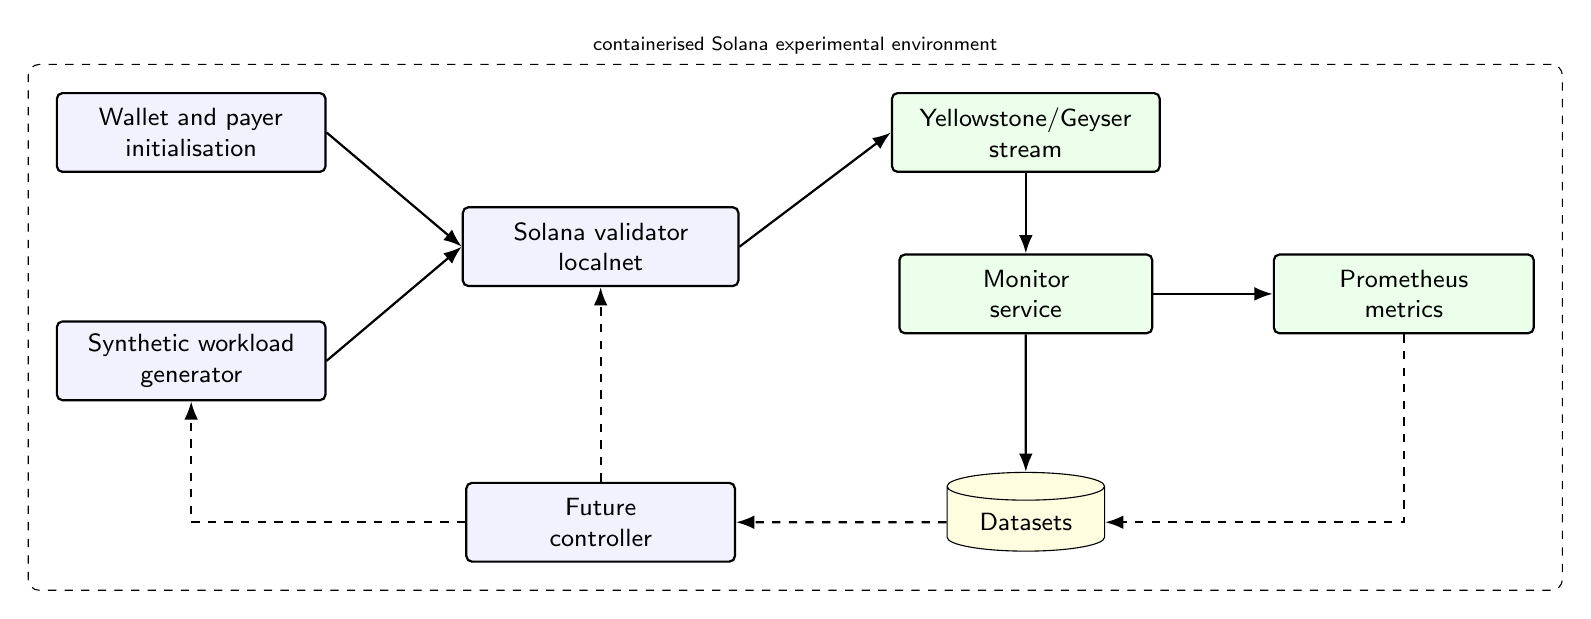
\begin{tikzpicture}[x=1cm,y=1cm]
\node[dboxwide, minimum width=3.4cm] (wallet) at (0,1.8) {Wallet and payer\\initialisation};
\node[dboxwide, minimum width=3.4cm] (load) at (0,-1.1) {Synthetic workload\\generator};
\node[dboxwide, minimum width=3.5cm] (validator) at (5.2,0.35) {Solana validator\\localnet};
\node[dobs, minimum width=3.4cm] (geyser) at (10.6,1.8) {Yellowstone/Geyser\\stream};
\node[dobs, minimum width=3.2cm] (monitor) at (10.6,-0.25) {Monitor\\service};
\node[dobs, minimum width=3.3cm] (prom) at (15.4,-0.25) {Prometheus\\metrics};
\node[dstore] (data) at (10.6,-3.15) {Datasets};
\node[dboxwide, minimum width=3.3cm] (controller) at (5.2,-3.15) {Future\\controller};
\draw[darrow] (wallet.east) -- (validator.west);
\draw[darrow] (load.east) -- (validator.west);
\draw[darrow] (validator.east) -- (geyser.west);
\draw[darrow] (geyser.south) -- (monitor.north);
\draw[darrow] (monitor.east) -- (prom.west);
\draw[darrow] (monitor.south) -- (data.north);
\draw[dfeedback] (prom.south) |- (data.east);
\draw[dfeedback] (data.west) -- (controller.east);
\draw[dfeedback] (controller.north) -- (validator.south);
\draw[dfeedback] (controller.west) -| (load.south);
\node[dframe, fit=(wallet)(load)(validator)(geyser)(monitor)(prom)(data)(controller), inner sep=0.35cm,
label={[font=\sffamily\scriptsize]above:containerised Solana experimental environment}] {};
\end{tikzpicture}%
}
\caption{High-level architecture of the Solana case-study testbed. Dashed arrows indicate the planned feedback-control extension.}
\label{fig:solana-architecture}
\end{figure}

\subsection{Component responsibilities}
\label{subsec:components}

\Cref{tab:components} maps the major components to their research roles. The design principle is to keep each component observable and replaceable. For example, a simple shell-based workload generator may later be replaced with a Python generator, a Rust generator, or a controller-driven generator without changing the validator container itself.

\begin{table}[H]
\centering
\caption{Component responsibilities in the Solana testbed}
\label{tab:components}
\begin{tabularx}{\textwidth}{L{3.3cm}Y Y}
\toprule
\textbf{Component} & \textbf{Responsibility} & \textbf{Research value} \\
\midrule
Validator container & Runs the private Solana localnet and exposes RPC and validator behaviour. & System under test. \\
Wallet initialisation & Creates or funds accounts required by experiments. & Reproducible experiment preparation. \\
Workload generator & Submits controlled transaction or RPC pressure. & Defines experimental input. \\
Yellowstone/Geyser & Streams validator-side events such as slots, transactions, blocks, or account updates. & Low-latency observability path. \\
Monitor container & Collects, transforms, and exports selected metrics. & Converts events into datasets and monitoring signals. \\
Prometheus endpoint & Exposes scrapeable time-series metrics. & Enables standard monitoring and later control input. \\
Dataset output & Stores raw and derived metrics with metadata. & Supports replication, analysis, and publication. \\
Controller interface & Adjusts workload or configuration based on observed state. & Planned closed-loop extension. \\
\bottomrule
\end{tabularx}
\end{table}

\subsection{Observability through Geyser and Yellowstone}
\label{subsec:geyser}

The Geyser interface is central because it allows validator-side state changes to be exported to external systems. The Agave documentation explains that the validator supports a plugin mechanism for transmitting information about accounts, slots, blocks, and transactions to external stores such as relational databases, NoSQL databases, or Kafka \cite{anza2026geyser}. The Yellowstone gRPC repository describes a Geyser-based gRPC interface for Solana with plugin and sample clients, providing streams for slots, blocks, transactions, and account update notifications over a standardised path \cite{rpcpool2026yellowstone}. In the proposed testbed, this streaming layer is not merely a data export convenience; it is part of the benchmark design.

\begin{figure}[H]
\centering
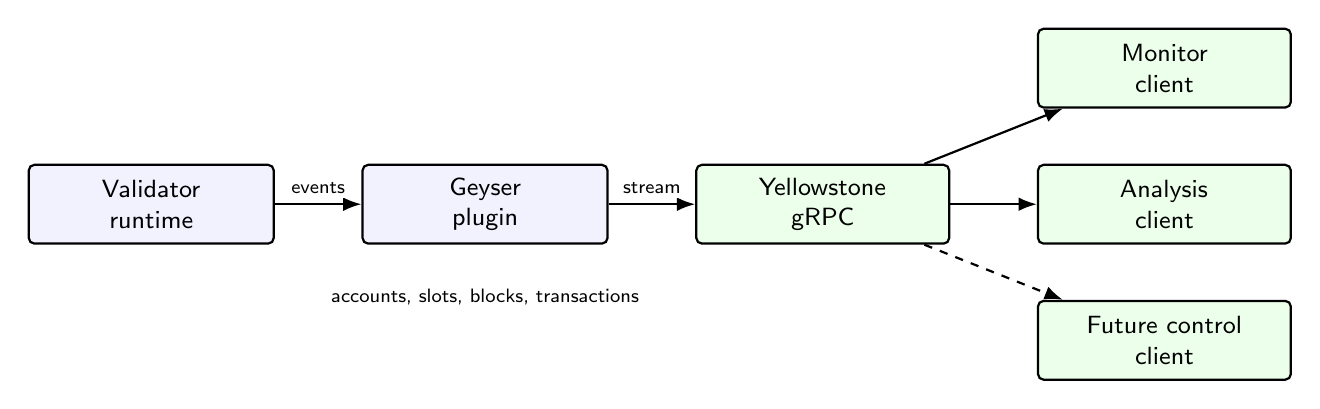
\begin{tikzpicture}
\node[dbox] (validator) {Validator\\runtime};
\node[dbox, right=1.1cm of validator] (plugin) {Geyser\\plugin};
\node[dobs, right=1.1cm of plugin] (grpc) {Yellowstone\\gRPC};
\node[dobs, above right=0.7cm and 1.1cm of grpc] (client1) {Monitor\\client};
\node[dobs, right=1.1cm of grpc] (client2) {Analysis\\client};
\node[dobs, below right=0.7cm and 1.1cm of grpc] (client3) {Future control\\client};

\draw[darrow] (validator) -- node[dnote, above=2pt] {events} (plugin);
\draw[darrow] (plugin) -- node[dnote, above=2pt] {stream} (grpc);
\draw[darrow] (grpc) -- (client1);
\draw[darrow] (grpc) -- (client2);
\draw[dfeedback] (grpc) -- (client3);

\node[dnote, below=5mm of plugin] {accounts, slots, blocks, transactions};
\end{tikzpicture}
\caption{Role of Geyser and Yellowstone gRPC in the observability path.}
\label{fig:geyser-path}
\end{figure}


\section{Implementation boundary and claim status}
\label{sec:implementation-boundary}

A central risk in testbed papers is overclaiming. A repository, a localnet, and an observability extension do not automatically justify claims about production performance, mainnet behaviour, or the effectiveness of adaptive controllers. This section therefore separates the current article's methodological claims from claims that require future experimental evidence.

\begin{table}[H]
\centering
\small
\caption{Implementation boundary for the current article version}
\label{tab:implementation-boundary}
\begin{tabularx}{\textwidth}{L{3.1cm}Y Y}
\toprule
\textbf{Area} & \textbf{Status in this article} & \textbf{Interpretation for claims} \\
\midrule
Conceptual model & Included as the main theoretical contribution. & Claims may be made about methodology and design rationale. \\
Containerised Solana localnet & Treated as the case-study foundation and linked to public artefacts. & Claims should be limited to reproducible local experimental infrastructure unless measured data are added. \\
Yellowstone/Geyser observability & Treated as an observability-path extension and research direction supported by referenced artefacts. & Claims may describe architecture and intended observability role; quantitative overhead claims require experiments. \\
Prometheus-compatible metrics & Included as part of the target monitoring architecture. & Claims should focus on metric taxonomy and dataset design until real scrape data are included. \\
Synthetic workload generator & Included as a required component of the benchmark design. & Workload realism, transaction success, and latency claims require defined workload profiles and recorded runs. \\
Dataset publication & Included as a publication model and metadata requirement. & Dataset claims require concrete files, checksums, host metadata, and release identifiers. \\
Feedback controller & Explicitly treated as future work. & No claim should be made that control, optimisation, RL, or MARL has already been validated. \\
Kubernetes and multi-validator scaling & Explicitly treated as future work. & The current paper should not generalise single-host results to cluster-level behaviour. \\
\bottomrule
\end{tabularx}
\end{table}

The practical consequence is that the present manuscript should be read as a methodological, artefact-oriented, and experiment-design paper. Its strongest current claims concern framing, requirements, architecture, reproducibility discipline, and the experimental roadmap. Strong empirical claims should be added only after the corresponding datasets and validation scripts are available.


\section{Experimental design}
\label{sec:experimental-design}

The purpose of the experimental design is to make the future empirical version of the article executable rather than merely aspirational. Each experiment should identify the independent variable being manipulated, the dependent variables being measured, the artefacts required for replication, and the claim that the experiment is allowed to support. This discipline is especially important for a local blockchain testbed, because small differences in host hardware, container image, ledger reset policy, or observability configuration can change the interpretation of the results.

The design assumes an incremental path. Baseline boot experiments should be completed first, because later workload and observability claims are not meaningful if the localnet cannot be started reproducibly. Transaction-load and RPC-pressure experiments should then exercise the system under controlled synthetic demand. Observability-overhead and Geyser stream-latency experiments should quantify the cost and value of the telemetry path. Resource-constrained and cross-host experiments should test robustness and reproducibility. Finally, control-readiness experiments should prepare the environment for rule-based or classical feedback baselines before any learning-based controller is introduced.

\subsection{Experimental matrix}
\label{subsec:experimental-matrix}

\Cref{tab:experimental-matrix} defines the proposed experimental matrix. The matrix is not a results table. It is a design table: it states what must be run and recorded before the article can make stronger empirical claims.

\begin{table}[H]
\centering
\caption{Experimental matrix for future empirical versions}
\label{tab:experimental-matrix}
\begin{tabularx}{\textwidth}{L{2.7cm}Y Y Y}
\toprule
\textbf{Experiment} & \textbf{Independent variable} & \textbf{Dependent variables} & \textbf{Required artefact} \\
\midrule
Baseline boot & Container image version, compose file, ledger reset policy. & RPC health, slot progression, startup time, container exit status. & Boot log, health-check transcript, baseline metrics CSV, metadata JSON. \\
Transaction load & Target transaction rate, burst profile, duration, account set, random seed. & Submission count, confirmation count, failure rate, confirmation latency, CPU and memory use. & Workload log, transaction summary CSV, time-series metrics, workload profile file. \\
RPC pressure & RPC request rate, request mix, concurrency, duration. & RPC latency, error rate, validator health, resource pressure. & RPC pressure log, response-latency CSV, validator-health timeline. \\
Observability overhead & Geyser and monitor enabled or disabled; Prometheus scrape interval. & CPU delta, memory delta, latency delta, throughput delta, event-processing delay. & Paired-run metrics, overhead comparison table, run-pair metadata. \\
Geyser stream latency & Event type, monitor client configuration, timestamp source. & Validator event count, monitor receive time, stream delay, missing events. & Event trace CSV, timestamp alignment notes, stream integrity report. \\
Resource-constrained run & CPU quota, memory limit, disk mode, network constraint where available. & Throughput, latency, errors, restart count, recovery time. & Constraint configuration, container stats, failure/recovery timeline. \\
Cross-host reproducibility & Hostname, CPU, memory, OS, kernel, container engine. & Metric variance across hosts, reproducibility of pass/fail status, distributional differences. & Host metadata JSON files, cross-host comparison CSV, reproducibility summary. \\
Control-readiness run & Scripted workload adjustment rule or configuration effector. & Response time, stability, safety violations, recovery behaviour. & Controller transcript, before/after metrics, safety-event log. \\
\bottomrule
\end{tabularx}
\end{table}

\subsection{Run profiles and sequencing}
\label{subsec:run-profiles}

The experiments should be executed through named run profiles. A profile should be a small, version-controlled description of the workload, duration, observability settings, and expected outputs. A recommended sequence is:

\begin{enumerate}
  \item \textbf{boot-baseline}: start the validator and confirm health without synthetic load.
  \item \textbf{txload-low}: run a conservative transaction-load profile to validate instrumentation.
  \item \textbf{txload-step}: increase the target rate in stages to observe latency and resource response.
  \item \textbf{rpc-pressure}: apply read/query pressure separately from transaction submission.
  \item \textbf{obs-off} and \textbf{obs-on}: run paired profiles for observability-overhead estimation.
  \item \textbf{geyser-latency}: measure event propagation through the Geyser/Yellowstone path.
  \item \textbf{resource-limit}: repeat a known workload under constrained CPU or memory.
  \item \textbf{cross-host}: repeat selected profiles on at least two hosts using identical code and image digests.
\end{enumerate}

For each profile, the article should preserve a distinction between \emph{input parameters}, \emph{measured signals}, and \emph{derived summaries}. Input parameters belong in version-controlled profile files. Measured signals belong in raw datasets. Derived summaries and figures should be reproducible from scripts.

\subsection{Claim-to-experiment mapping}
\label{subsec:claim-experiment-mapping}

The experimental design should constrain the strength of future claims. For example, a baseline boot run can support a claim that the localnet starts reproducibly under specified conditions. It cannot support a claim about transaction latency. A paired observability-overhead run can support a claim about the overhead of a specific monitoring configuration on a specific host. It cannot support a general claim about all Geyser deployments. A cross-host run can support a limited reproducibility claim only if host metadata, image digests, and workload profiles are published alongside the metrics.

This claim-to-experiment mapping is deliberately conservative. Its purpose is to make the paper easier to defend in review and easier to extend when real datasets become available.


\section{Preliminary empirical pilot}
\label{sec:empirical-pilot}

The preceding sections define the experimental design and claim discipline required for empirical work. This section adds a preliminary pilot dataset to validate the measurement pipeline. The pilot is intentionally modest: it is a single-host, single-validator localnet study conducted on the host recorded as \texttt{fedora\_}, with all included runs using the same Git short commit \texttt{d0c848a}. The purpose is not to establish general Solana performance limits. The purpose is to test whether the proposed dataset structure can distinguish baseline localnet operation from controlled transaction-load profiles while preserving run metadata, validator health samples, RPC counters, and workload-side transaction evidence.

The pilot includes nine valid runs: three baseline runs, three low transaction-load runs, and three medium transaction-load runs. A previously collected \texttt{txload-low} archive without independent workload evidence is excluded from this pilot and treated as a diagnostic run rather than as transaction-load evidence.

\begin{table}[H]
\centering
\caption{Pilot dataset composition}
\label{tab:pilot-composition}
\begin{tabularx}{\textwidth}{L{3.0cm}L{2.0cm}Y Y}
\toprule
\textbf{Profile} & \textbf{Runs} & \textbf{Workload evidence} & \textbf{Permitted interpretation} \\
\midrule
Baseline & 3 & No external transaction generator. & Validator health and localnet progression under the default containerised configuration. \\
\texttt{txload-low} & 3 & Sequential SOL transfers generated from inside the validator container at target 1 transaction per second. & Low synthetic transaction pressure and workload-side success evidence. \\
\texttt{txload-medium} & 3 & Sequential SOL transfers generated from inside the validator container at target 2 transactions per second. & Higher synthetic transaction pressure, constrained by sequential CLI confirmation behaviour. \\
\bottomrule
\end{tabularx}
\end{table}

\Cref{tab:pilot-run-summary} reports the run-level summary. Each run has 60 RPC samples collected at five-second intervals. All included samples returned healthy validator status. The transaction-load profiles also include a workload-side transaction log, with attempted, successful, and failed transaction counts.

\begin{table}[H]
\centering
\caption{Run-level empirical pilot summary}
\label{tab:pilot-run-summary}
\begin{tabularx}{\textwidth}{L{3.1cm}L{1.5cm}L{1.4cm}L{1.4cm}L{1.6cm}L{1.8cm}L{1.5cm}L{1.4cm}}
\toprule
\textbf{Run timestamp} & \textbf{Profile} & \textbf{Health} & \textbf{Slot $\Delta$} & \textbf{Tx count $\Delta$} & \textbf{Workload ok} & \textbf{Failed} & \textbf{Mean ms} \\
\midrule
2026-05-15 11:15 & baseline & 60/60 & 759 & 759 & -- & -- & -- \\
2026-05-15 11:37 & baseline & 60/60 & 758 & 758 & -- & -- & -- \\
2026-05-15 11:47 & baseline & 60/60 & 768 & 768 & -- & -- & -- \\
2026-05-15 12:46 & low & 60/60 & 734 & 1000 & 265 & 0 & 791.3 \\
2026-05-15 13:25 & low & 60/60 & 733 & 998 & 264 & 0 & 798.1 \\
2026-05-15 14:17 & low & 60/60 & 735 & 992 & 263 & 0 & 796.5 \\
2026-05-15 13:14 & medium & 60/60 & 741 & 1102 & 360 & 0 & 763.2 \\
2026-05-15 13:32 & medium & 60/60 & 739 & 1102 & 362 & 0 & 760.3 \\
2026-05-15 14:24 & medium & 60/60 & 736 & 1096 & 358 & 0 & 767.1 \\
\bottomrule
\end{tabularx}
\end{table}

\begin{table}[H]
\centering
\caption{Profile-level empirical pilot summary}
\label{tab:pilot-profile-summary}
\begin{tabularx}{\textwidth}{L{2.7cm}L{1.2cm}L{1.5cm}L{1.6cm}L{1.8cm}L{1.8cm}L{1.8cm}L{1.8cm}}
\toprule
\textbf{Profile} & \textbf{Runs} & \textbf{Health} & \textbf{Mean slot $\Delta$} & \textbf{Mean tx $\Delta$} & \textbf{Mean workload ok} & \textbf{Achieved tx/s} & \textbf{Mean p95 ms} \\
\midrule
baseline & 3 & 180/180 & 761.7 & 761.7 & -- & -- & -- \\
\texttt{txload-low} & 3 & 180/180 & 734.0 & 996.7 & 264.0 & 0.94 & 887.3 \\
\texttt{txload-medium} & 3 & 180/180 & 738.7 & 1100.0 & 360.0 & 1.29 & 844.3 \\
\bottomrule
\end{tabularx}
\end{table}

\begin{figure}[H]
\centering
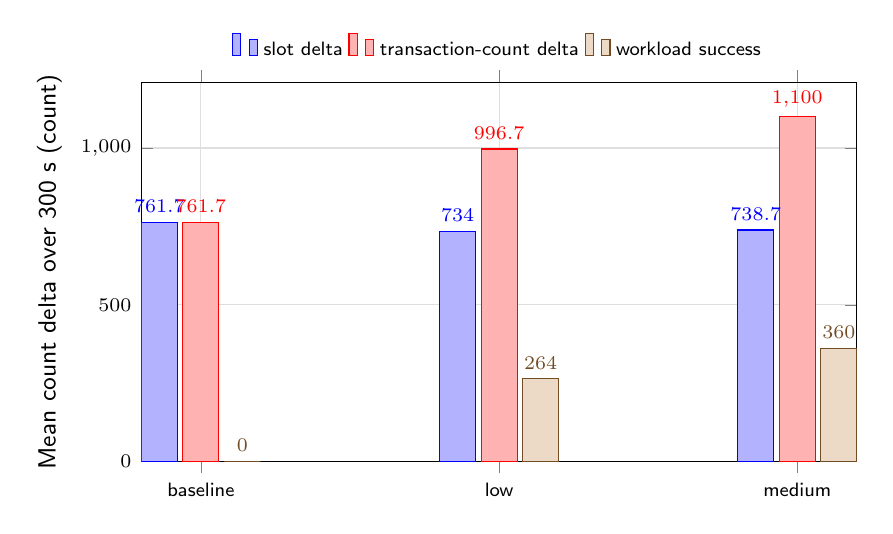
\begin{tikzpicture}
\begin{axis}[
  ybar,
  width=0.88\textwidth,
  height=6.4cm,
  bar width=13pt,
  ymin=0,
  ylabel={Mean count delta over 300 s (count)},
  symbolic x coords={baseline,low,medium},
  xtick=data,
  tick label style={font=\sffamily\scriptsize},
  label style={font=\sffamily\small},
  legend style={font=\sffamily\scriptsize, draw=none, fill=white, at={(0.5,1.03)}, anchor=south, legend columns=3},
  nodes near coords,
  every node near coord/.append style={font=\sffamily\scriptsize},
  grid=major,
  major grid style={draw=gray!25}
]
\addplot coordinates {(baseline,761.7) (low,734.0) (medium,738.7)};
\addplot coordinates {(baseline,761.7) (low,996.7) (medium,1100.0)};
\addplot coordinates {(baseline,0) (low,264.0) (medium,360.0)};
\legend{slot delta, transaction-count delta, workload success}
\end{axis}
\end{tikzpicture}
\caption{Mean slot progression, transaction-count progression, and workload-side successes in the pilot dataset. The figure is intended to validate measurement separability rather than to rank Solana performance.}
\label{fig:pilot-profile-deltas}
\end{figure}

The main finding is methodological. In the baseline runs, the transaction-count delta is approximately equal to the slot delta. In the transaction-load profiles, the transaction-count delta is greater than the slot delta by an amount that is consistent with the workload-side successful transfer counts. For the low profile, the mean transaction-count delta is 996.7 while the mean workload-side success count is 264.0. For the medium profile, the corresponding values are 1100.0 and 360.0. This alignment indicates that the collection pipeline can connect an externally named workload profile, validator RPC counters, and workload-side transaction evidence.

The pilot also exposes an important engineering limitation. The workload generator used sequential \texttt{solana transfer} commands and waited for transaction confirmation. Consequently, the achieved rates were lower than the nominal target rates: approximately 0.94 transactions per second for the low profile and 1.29 transactions per second for the medium profile. This is acceptable for the present pilot because the goal is not saturation. It does, however, show that future higher-pressure experiments should use an asynchronous or batched workload generator rather than sequential CLI transfers.

\subsection{Pilot claim boundary}
\label{subsec:pilot-claim-boundary}

The pilot supports four limited claims. First, the localnet remained healthy throughout the included 300-second runs. Second, the dataset bundle format is sufficient to preserve host metadata, Git identity, compose files, RPC metrics, and workload evidence. Third, low and medium synthetic transaction-load profiles are distinguishable from baseline behaviour in transaction-count deltas. Fourth, the workload-side success counts are consistent with the additional RPC-level transaction-count progression.

The pilot does not support claims about public Solana mainnet performance, multi-validator behaviour, Geyser stream latency, observability overhead, or controller performance. Those claims require the additional experiments described in the experimental matrix. The next empirical extension should therefore add paired observability-on/off runs and a higher-quality workload generator before making stronger performance claims.

\section{Experimental protocol and metric taxonomy}
\label{sec:protocol}

A useful experimental protocol must separate the scientific question, workload profile, system configuration, metric collection, and dataset publication. The protocol should also record enough context to make the experiment reproducible on another host.

\subsection{Experiment classes}
\label{subsec:experiment-classes}

\Cref{tab:experiment-classes} defines a minimal set of experiment classes for the next version of the testbed paper. These experiments are intentionally staged. The first group validates reproducibility. The second group measures behaviour under synthetic workload. The third group evaluates the cost and value of observability. The fourth group prepares the system for feedback control.

\begin{table}[H]
\centering
\caption{Proposed experiment classes}
\label{tab:experiment-classes}
\begin{tabularx}{\textwidth}{L{3.0cm}Y Y Y}
\toprule
\textbf{Experiment class} & \textbf{Purpose} & \textbf{Main signals} & \textbf{Expected output} \\
\midrule
Baseline boot & Validate reproducible localnet startup. & Health status, slot progression, RPC availability. & Pass/fail log and baseline metrics. \\
Transaction load & Evaluate controlled synthetic transaction pressure. & Submission rate, success rate, latency, resource use. & Time-series dataset and summary table. \\
RPC pressure & Study validator responsiveness under read/query load. & RPC latency, error rate, validator health. & Responsiveness profile. \\
Observability overhead & Compare runs with and without monitoring/Geyser. & CPU, memory, latency, event delay. & Overhead estimate. \\
Geyser stream latency & Estimate event propagation delay through the observability path. & Event timestamp differences, queueing behaviour. & Stream latency dataset. \\
Resource constraint & Evaluate behaviour under CPU or memory limits. & Throughput, latency, failures, recovery time. & Perturbation profile. \\
Dataset reproducibility & Repeat selected runs across hosts. & Metric distributions, host metadata, variance. & Cross-host comparison table. \\
Control readiness & Test scripted or rule-based adjustment. & Response to workload changes and safety violations. & Baseline for future controllers. \\
\bottomrule
\end{tabularx}
\end{table}

\begin{figure}[H]
\centering
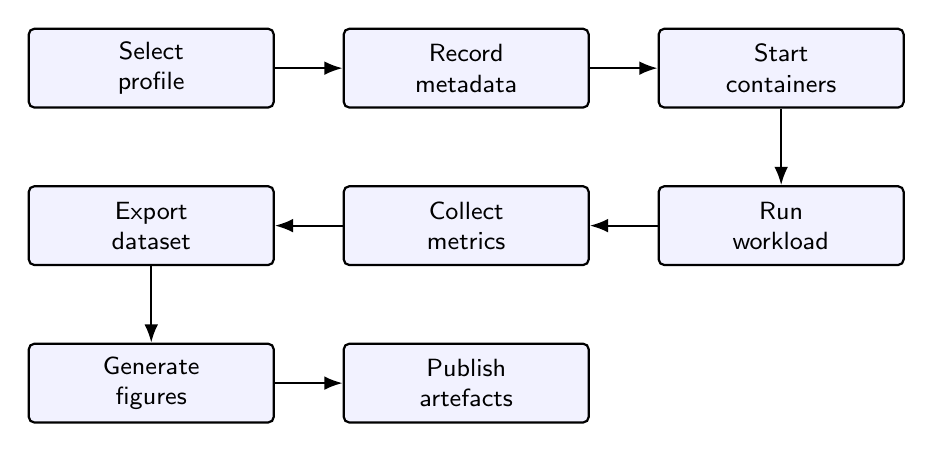
\begin{tikzpicture}[x=1cm,y=1cm]
\node[dbox] (s1) at (0,0) {Select\\profile};
\node[dbox] (s2) at (4.0,0) {Record\\metadata};
\node[dbox] (s3) at (8.0,0) {Start\\containers};
\node[dbox] (s4) at (8.0,-2.0) {Run\\workload};
\node[dbox] (s5) at (4.0,-2.0) {Collect\\metrics};
\node[dbox] (s6) at (0,-2.0) {Export\\dataset};
\node[dbox] (s7) at (0,-4.0) {Generate\\figures};
\node[dbox] (s8) at (4.0,-4.0) {Publish\\artefacts};

\draw[darrow] (s1.east) -- (s2.west);
\draw[darrow] (s2.east) -- (s3.west);
\draw[darrow] (s3.south) -- (s4.north);
\draw[darrow] (s4.west) -- (s5.east);
\draw[darrow] (s5.west) -- (s6.east);
\draw[darrow] (s6.south) -- (s7.north);
\draw[darrow] (s7.east) -- (s8.west);
\end{tikzpicture}
\caption{Recommended experiment lifecycle for dataset-producing benchmark runs.}
\label{fig:experiment-lifecycle}
\end{figure}

\subsection{Metric taxonomy}
\label{subsec:metric-taxonomy}

The testbed should avoid reducing performance to one metric. Throughput and latency remain important, but they must be interpreted together with validator health, observability delay, RPC responsiveness, and resource consumption.

\begin{table}[H]
\centering
\caption{Metric taxonomy for the Solana testbed}
\label{tab:metric-taxonomy}
\begin{tabularx}{\textwidth}{L{3.3cm}Y Y}
\toprule
\textbf{Metric group} & \textbf{Examples} & \textbf{Interpretation} \\
\midrule
Workload input & Target rate, burst size, request mix, duration, random seed. & What the experiment asked the system to do. \\
Transaction outcome & Submitted, confirmed, failed, retried, dropped. & Whether the workload succeeded. \\
Latency & Submission latency, confirmation latency, RPC response latency, stream delay. & User-visible and observability-path responsiveness. \\
Validator state & Health status, slot progression, block or transaction event counts. & Internal progress of the localnet. \\
Geyser stream & Event count, stream gaps, client receive time, monitor processing time. & Observability-path behaviour. \\
Container resources & CPU, memory, network I/O, disk I/O, restart count. & Runtime resource pressure. \\
Host metadata & Hostname, CPU model, memory, OS, kernel, container engine. & Reproducibility and cross-host analysis. \\
Build metadata & Git commit, image tag, image digest, Solana version, compose file. & Artefact traceability. \\
\bottomrule
\end{tabularx}
\end{table}

\begin{figure}[H]
\centering
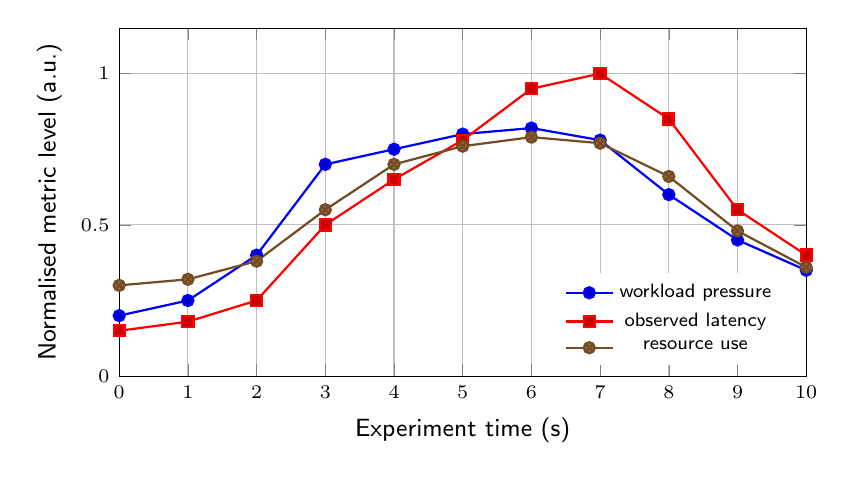
\begin{tikzpicture}
\begin{axis}[
  width=0.85\textwidth,
  height=6cm,
  tick label style={font=\sffamily\scriptsize},
  label style={font=\sffamily\small},
  legend style={font=\sffamily\scriptsize, draw=none, fill=white},
  xlabel={Experiment time (s)},
  ylabel={Normalised metric level (a.u.)},
  xmin=0, xmax=10,
  ymin=0, ymax=1.15,
  legend pos=south east,
  grid=both,
  every axis plot/.append style={thick}
]
\addplot coordinates {(0,0.2) (1,0.25) (2,0.4) (3,0.7) (4,0.75) (5,0.8) (6,0.82) (7,0.78) (8,0.6) (9,0.45) (10,0.35)};
\addlegendentry{workload pressure}
\addplot coordinates {(0,0.15) (1,0.18) (2,0.25) (3,0.5) (4,0.65) (5,0.78) (6,0.95) (7,1.0) (8,0.85) (9,0.55) (10,0.4)};
\addlegendentry{observed latency}
\addplot coordinates {(0,0.3) (1,0.32) (2,0.38) (3,0.55) (4,0.7) (5,0.76) (6,0.79) (7,0.77) (8,0.66) (9,0.48) (10,0.36)};
\addlegendentry{resource use}
\end{axis}
\end{tikzpicture}
\caption{Illustrative time-series view for multi-metric interpretation. The values are schematic placeholders rather than measured results.}
\label{fig:illustrative-timeseries}
\end{figure}

\subsection{Dataset naming and metadata}
\label{subsec:dataset-naming}

Dataset files should be self-describing enough to remain useful outside the original machine. A recommended naming pattern is:

\begin{quote}\small
\texttt{YYYYMMDDTHHMMSSZ\_hostname\_profile\_duration\_gitshortsha\_metrics.csv}
\end{quote}

For example:

\begin{quote}\small
\texttt{20260515T121500Z\_hpz440\_txload-low\_300s\_a1b2c3d\_metrics.csv}
\end{quote}

The file name should not replace a metadata sidecar file. Each dataset should also include a structured metadata record such as JSON or YAML.

\begin{table}[H]
\centering
\caption{Recommended dataset metadata fields}
\label{tab:metadata}
\begin{tabularx}{\textwidth}{L{3.5cm}Y Y}
\toprule
\textbf{Field group} & \textbf{Fields} & \textbf{Reason} \\
\midrule
Run identity & run id, timestamp, hostname, operator, project version. & Distinguish repeated runs. \\
Source identity & Git repository, commit hash, branch, dirty flag. & Link dataset to code state. \\
Image identity & Container image tags, image digests, compose file. & Recreate runtime environment. \\
Host identity & CPU model, memory, OS, kernel, container engine version. & Explain cross-host differences. \\
Workload identity & Profile name, rate, duration, seed, request mix. & Reproduce input pressure. \\
Solana identity & Solana/Agave version, validator flags, ledger mode. & Reproduce system under test. \\
Observability identity & Geyser config, monitor version, Prometheus scrape interval. & Interpret telemetry path. \\
Output identity & Raw files, derived files, figure files, checksum. & Validate publication artefacts. \\
\bottomrule
\end{tabularx}
\end{table}


\section{Evidence plan for empirical versions}
\label{sec:evidence-plan}

The current article now includes a preliminary empirical pilot, but it remains conservative about generalisation. A later results-oriented version should connect every stronger substantive claim to a dataset, metric, and reproducibility record. \Cref{tab:evidence-plan} defines a practical evidence plan.

\begin{table}[H]
\centering
\caption{Evidence plan for converting methodological claims into empirical claims}
\label{tab:evidence-plan}
\begin{tabularx}{\textwidth}{L{3.4cm}Y Y L{2.5cm}}
\toprule
\textbf{Claim type} & \textbf{Required evidence} & \textbf{Primary metric or artefact} & \textbf{Current status} \\
\midrule
Reproducible startup & Repeated clean launches on at least one host, with recorded versions and logs. & Validator health, slot progression, RPC availability, compose file, image digest. & Pilot evidence included. \\
Workload handling & Runs with defined synthetic transaction or RPC profiles. & Submission rate, success rate, confirmation latency, error count. & Pilot evidence included. \\
Observability path function & Evidence that Yellowstone/Geyser events are received and transformed by monitor components. & Event counts, stream timestamps, monitor receive times, missing-event checks. & Architecture defined. \\
Observability overhead & Paired runs with and without observability components. & CPU, memory, latency, throughput, stream delay. & Future experiment. \\
Cross-host reproducibility & Repeated profiles on two or more machines. & Hostname-aware metric distributions and metadata sidecars. & Future experiment. \\
Dataset traceability & Published raw data, derived data, scripts, figures, and checksums. & DOI records, Git commit hash, checksums, README mapping. & Pilot bundle validated; publication pending. \\
Rule-based control readiness & Scripted adjustment of workload or configuration using observed state. & Response time, safety violations, stability, recovery behaviour. & Future work. \\
RL or MARL suitability & Baselines, environment definition, reward design, and safety constraints. & Baseline comparison, training logs, evaluation seeds, policy robustness. & Long-term roadmap. \\
\bottomrule
\end{tabularx}
\end{table}

This evidence plan also protects the article from premature generalisation. It makes clear which claims are already supported by design artefacts and which require future data collection.

\section{Data requirements for future empirical extension}
\label{sec:data-requirements}

The current manuscript includes a small empirical pilot, but additional empirical data become necessary when the manuscript is revised to make stronger measured claims about performance, observability overhead, Geyser/Yellowstone latency, cross-host reproducibility, or controller behaviour. This distinction is important because it separates the validity of the proposed research infrastructure and pilot pipeline from the validity of future numerical results.

\Cref{tab:data-readiness} defines the practical trigger points for requesting datasets. It should be read as an editorial control mechanism: if a claim remains architectural or methodological, the current artefacts, protocols, and pilot dataset are sufficient; if a claim becomes broader or more quantitative, the corresponding run bundle must be collected and archived.

\begin{table}[H]
\centering
\caption{When empirical data become required}
\label{tab:data-readiness}
\begin{tabularx}{\textwidth}{L{3.4cm}Y Y}
\toprule
\textbf{Manuscript claim} & \textbf{Data requirement} & \textbf{Minimum acceptable input} \\
\midrule
Methodological claim about benchmark evolution & No new dataset required. & Literature-supported argument and conceptual diagrams. \\
Architectural claim about the Solana testbed & No performance dataset required, but repository state must match the text. & Current compose files, README, release notes, and DOI records. \\
Claim that the localnet starts reproducibly & Baseline boot data required. & At least three clean boot runs with health checks, slot progression, logs, and metadata. \\
Claim about transaction-load behaviour & Transaction-load dataset required. & Low and medium load profiles with latency, success rate, errors, CPU, memory, and run metadata. \\
Claim about observability overhead & Paired comparison required. & Matched runs with observability disabled and enabled, using the same workload and host. \\
Claim about Geyser or Yellowstone latency & Stream-timing dataset required. & Event timestamps, monitor receive timestamps, stream counts, and missing-event checks. \\
Claim about cross-host reproducibility & Multi-host dataset required. & The same profile executed on at least two hostnames with complete host metadata. \\
Claim about feedback control & Controller-run dataset required. & Baseline open-loop run, rule-based run, safety conditions, controller logs, and recovery metrics. \\
\bottomrule
\end{tabularx}
\end{table}

For a first empirical revision, the most efficient dataset package would contain three baseline runs and two transaction-load profiles on one host. A stronger revision would add paired observability-overhead runs and one repeated profile on a second host. Learning-based control data should not be collected until open-loop, scripted, and rule-based baselines are stable.

\section{Research artefacts and publication model}
\label{sec:artefacts}

Reproducible benchmarking should publish not only the article but also the code, configuration, datasets, and derived figures. The Solana project already has a public GitHub repository and DOI-backed Zenodo records referenced from the repository README \cite{okhoshaba2026repo}. This creates a foundation for a stronger research \artifact{} model.

\begin{table}[H]
\centering
\caption{Current and planned artefact classes}
\label{tab:artefacts}
\begin{tabularx}{\textwidth}{L{3.0cm}Y Y}
\toprule
\textbf{Artefact class} & \textbf{Current role} & \textbf{Recommended next step} \\
\midrule
GitHub repository & Source code, compose files, scripts, documentation. & Ensure README status, release notes, and article claims are synchronised. \\
Zenodo software record & Persistent reference for versioned software state. & Use DOI in article and preserve exact release archive. \\
Zenodo technical note & Persistent explanation of design and validation state. & Link technical note to article methodology. \\
Raw datasets & Evidence from individual benchmark runs. & Include hostname and metadata sidecars. \\
Derived datasets & Cleaned or aggregated results. & Publish processing scripts with checksums. \\
Figures & Visual evidence used in article. & Generate from scripts rather than manual editing. \\
Experiment protocol & Exact run procedure. & Store as markdown and LaTeX appendix. \\
\bottomrule
\end{tabularx}
\end{table}

\begin{figure}[H]
\centering
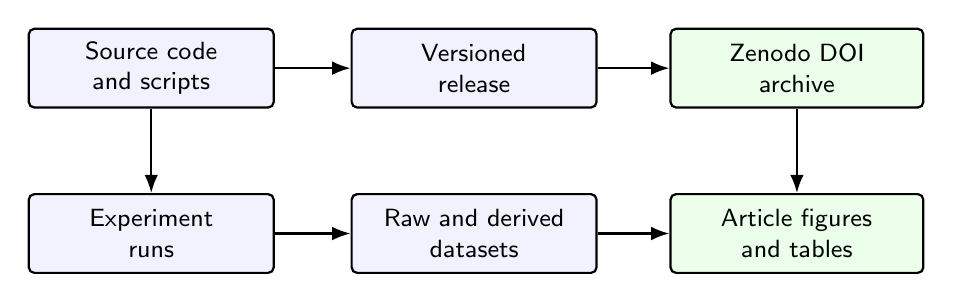
\begin{tikzpicture}[x=1cm,y=1cm]
\node[dbox] (code) at (0,0) {Source code\\and scripts};
\node[dbox] (release) at (4.1,0) {Versioned\\release};
\node[dobs] (zenodo) at (8.2,0) {Zenodo DOI\\archive};
\node[dbox] (runs) at (0,-2.1) {Experiment\\runs};
\node[dbox] (datasets) at (4.1,-2.1) {Raw and derived\\datasets};
\node[dobs] (paper) at (8.2,-2.1) {Article figures\\and tables};

\draw[darrow] (code.east) -- (release.west);
\draw[darrow] (release.east) -- (zenodo.west);
\draw[darrow] (code.south) -- (runs.north);
\draw[darrow] (runs.east) -- (datasets.west);
\draw[darrow] (datasets.east) -- (paper.west);
\draw[darrow] (zenodo.south) -- (paper.north);
\end{tikzpicture}
\caption{Recommended publication pipeline linking repository, releases, datasets, and article evidence.}
\label{fig:publication-pipeline}
\end{figure}

Before submission, the repository should be checked for consistency between the implemented state and the article text. Any section describing planned work should be clearly separated from completed work. This is especially important where observability, monitoring, Docker Hub images, and DOI releases are mentioned, because readers may compare article claims directly with the repository.

\section{Repository integration strategy}
\label{sec:repository-integration}

The article should be integrated into the public repository as a maintained research artefact rather than as a detached manuscript. Repository integration has two purposes. First, it makes the article source, bibliography, build instructions, and generated PDF traceable to a specific project state. Second, it reduces the risk of divergence between the manuscript, README files, release notes, datasets, and Zenodo records.

The recommended integration model is conservative: keep the LaTeX source in a dedicated article directory, keep dataset templates and empirical datasets outside the article source tree, and link the article from the research-program documentation. The article should not become the only source of truth about implementation status. Instead, it should cite and summarise repository state that is also documented in README and release files.

\subsection{Recommended repository layout}
\label{subsec:repository-layout}

A practical layout is shown in \cref{tab:repository-layout}. The exact directory names may be adjusted to match the repository, but the separation of roles should be preserved: article source, project documentation, dataset specifications, empirical data, and publication records should remain distinguishable.

\begin{table}[H]
\centering
\caption{Recommended repository integration layout}
\label{tab:repository-layout}
\begin{tabularx}{\textwidth}{L{5.2cm}Y Y}
\toprule
\textbf{Path} & \textbf{Role} & \textbf{Policy} \\
\midrule
\path{paper/synthetic-benchmarks-solana/} & LaTeX source, bibliography, build instructions, and generated PDF for this article. & Commit source files and build notes. Commit PDF when useful for review or release. \\
\path{docs/research-program/} & Narrative project documentation and links to the article. & Keep short status pages here; avoid duplicating the full article. \\
\path{docs/research-program/article-status.md} & Human-readable status of article versions, claims, and next actions. & Update on each article milestone. \\
\path{data/raw/} & Future raw experimental outputs from validator, workload, monitor, and metrics runs. & Commit only small or curated data; use Zenodo for larger datasets. \\
\path{data/derived/} & Cleaned or aggregated datasets generated from raw data. & Regenerate from scripts where possible. \\
\path{results/figures/} & Generated figures from empirical data. & Store generated plots with script references. \\
\path{scripts/} & Build, validation, dataset collection, and plotting scripts. & Prefer deterministic scripts over manual figure editing. \\
\path{prompts/codex/} & Optional local Codex prompts for repository maintenance tasks. & Use for repeatable integration or documentation updates. \\
\path{releases/} or \path{docs/releases/} & Release notes and DOI mapping. & Keep GitHub and Zenodo identifiers synchronised. \\
\bottomrule
\end{tabularx}
\end{table}

\begin{figure}[H]
\centering
\resizebox{0.96\textwidth}{!}{%
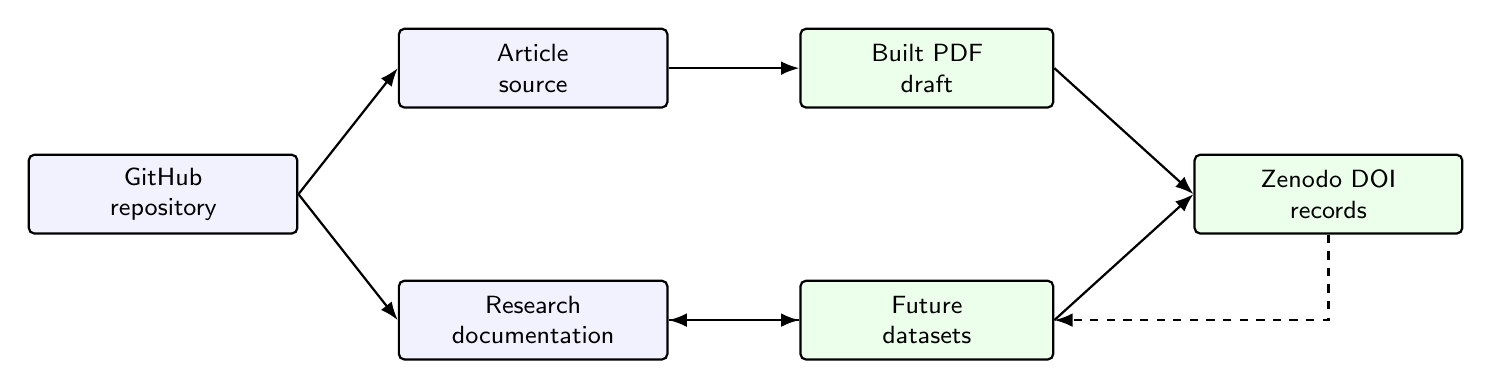
\begin{tikzpicture}[x=1cm,y=1cm]
\node[dboxwide, minimum width=3.0cm] (repo) at (0,0) {GitHub\\repository};
\node[dboxwide, minimum width=3.2cm] (article) at (4.7,1.6) {Article\\source};
\node[dboxwide, minimum width=3.2cm] (docs) at (4.7,-1.6) {Research\\documentation};
\node[dobs, minimum width=3.2cm] (pdf) at (9.7,1.6) {Built PDF\\draft};
\node[dobs, minimum width=3.2cm] (data) at (9.7,-1.6) {Future\\datasets};
\node[dobs, minimum width=3.4cm] (zenodo) at (14.8,0) {Zenodo DOI\\records};
\draw[darrow] (repo.east) -- (article.west);
\draw[darrow] (repo.east) -- (docs.west);
\draw[darrow] (article.east) -- (pdf.west);
\draw[darrow] (docs.east) -- (data.west);
\draw[darrow] (pdf.east) -- (zenodo.west);
\draw[darrow] (data.east) -- (zenodo.west);
\draw[dfeedback] (zenodo.south) |- (data.east);
\draw[dfeedback] (data.west) -- (docs.east);
\end{tikzpicture}%
}
\caption{Repository integration map for article source, documentation, generated PDF, future datasets, and DOI records.}
\label{fig:repository-integration}
\end{figure}

\subsection{Integration rules}
\label{subsec:integration-rules}

The following rules should be used when the article is committed to the repository.

\begin{enumerate}
  \item Keep the manuscript source in a dedicated article directory and avoid scattering LaTeX files across the repository.
  \item Treat the generated PDF as a review artefact. It may be committed for convenience, but the source files and build instructions are authoritative.
  \item Keep raw empirical data outside the article directory. The article should reference datasets; it should not become a data dump.
  \item Maintain a short status page that states the article version, current claim boundary, completed artefacts, missing empirical evidence, and next planned action.
  \item Update Zenodo and GitHub release references only when the repository state has actually been released or archived.
  \item When empirical datasets are added later, include metadata, host information, workload profiles, logs, and checksums before adding quantitative claims to the article.
\end{enumerate}

\subsection{Suggested integration commit}
\label{subsec:integration-commit}

A suitable first repository integration commit should be narrow and descriptive. It should add the article source, repository-facing README files, and status documentation, without claiming that empirical datasets are already available. A recommended commit message is:

\begin{quote}\small
\texttt{docs: add synthetic benchmarking article integration workflow}
\end{quote}

If the generated PDF is also committed, the commit body should say that the PDF is a derived review artefact generated from the LaTeX source. This prevents confusion about whether the PDF or the source is the maintained object.

\section{Operational GitHub integration workflow}
\label{sec:github-workflow}

The repository integration step should be performed as a small documentation-only change. Its purpose is to place the article and its supporting files into the repository, confirm that the manuscript can be rebuilt locally, inspect the staged changes, and push a narrow commit. It should not modify validator, wallet, monitor, container, or workload-generation implementation code.

The workflow in \cref{tab:github-workflow} assumes a local clone of the repository and an extracted article integration package. It deliberately separates copying files, building the PDF, inspecting the working tree, committing, and pushing. This separation makes the integration auditable and reversible.

\begin{table}[H]
\centering
\caption{Operational GitHub integration workflow}
\label{tab:github-workflow}
\begin{tabularx}{\textwidth}{L{3.2cm}Y Y}
\toprule
\textbf{Stage} & \textbf{Action} & \textbf{Expected result} \\
\midrule
Pre-flight & Confirm the repository branch, clean working tree, and location of the extracted integration package. & The user knows which branch will receive the article files. \\
Copy & Copy article source, PDF, build files, documentation, prompts, and scripts into their target paths. & New or updated files appear under \path{paper/}, \path{docs/research-program/}, \path{prompts/codex/}, and \path{scripts/}. \\
Build & Run the article build script from the repository root. & \path{paper/synthetic-benchmarks-solana/main.pdf} is regenerated successfully. \\
Inspect & Review \texttt{git status --short} and, when useful, \texttt{git diff --stat}. & Only article and documentation files are changed. \\
Stage files & Stage the article, documentation, prompt, and helper scripts explicitly. & No logs, temporary files, raw datasets, or implementation changes are staged by accident. \\
Commit & Commit with a documentation-oriented message. & The repository contains a traceable article integration commit. \\
Push & Push the branch to GitHub and verify it online. & GitHub shows the article source, review PDF, and status documentation. \\
\bottomrule
\end{tabularx}
\end{table}

A conservative command sequence is shown below. The paths should be adjusted to the local machine, but the ordering should be preserved.

\begin{verbatim}
# 1. Enter the local repository.
cd ~/project/solana-containerised-testbed

# 2. Confirm branch and cleanliness.
git branch --show-current
git status --short

# 3. Define the extracted integration package location.
PKG=~/Downloads/solana_benchmark_article_v1_1/repository-integration

# 4. Copy the article and repository-facing files.
bash "$PKG/scripts/integrate_synthetic_benchmark_article_v1_1.sh" \
  "$PKG" \
  "$(pwd)"

# 5. Rebuild the PDF from the repository copy.
bash scripts/build_synthetic_benchmarks_article.sh \
  paper/synthetic-benchmarks-solana

# 6. Inspect the working tree.
git status --short
git diff --stat

# 7. Stage only article and documentation files.
git add \
  paper/synthetic-benchmarks-solana \
  docs/research-program/synthetic-benchmarks-solana-article.md \
  docs/research-program/article-status.md \
  prompts/codex/21_github_integration_workflow_v1_1.md \
  scripts/build_synthetic_benchmarks_article.sh \
  scripts/integrate_synthetic_benchmark_article_v1_1.sh \
  scripts/check_synthetic_benchmark_article_integration.sh

# 8. Commit and push.
git commit -m "docs: add synthetic benchmarking article integration workflow"
git push
\end{verbatim}

The helper integration script is intentionally limited. It copies files into documentation and article paths, makes helper scripts executable, and prints the resulting status. It does not commit, push, delete datasets, or change runtime implementation files. The final decision about staging and committing remains with the repository maintainer.

\subsection{Rollback and safety checks}
\label{subsec:github-rollback}

If the integration was copied into the wrong branch or wrong repository, the change should be reverted before staging or committing. A safe rollback before committing is:

\begin{verbatim}
git restore --staged \
  paper/synthetic-benchmarks-solana \
  docs/research-program \
  prompts/codex \
  scripts/build_synthetic_benchmarks_article.sh \
  scripts/integrate_synthetic_benchmark_article_v1_1.sh \
  scripts/check_synthetic_benchmark_article_integration.sh

git restore \
  paper/synthetic-benchmarks-solana \
  docs/research-program \
  prompts/codex \
  scripts/build_synthetic_benchmarks_article.sh \
  scripts/integrate_synthetic_benchmark_article_v1_1.sh \
  scripts/check_synthetic_benchmark_article_integration.sh
\end{verbatim}

For newly added untracked files, inspect them first and then remove only the intended paths. Avoid broad cleanup commands unless the working tree has been reviewed carefully.

\begin{verbatim}
git status --short
rm -rf paper/synthetic-benchmarks-solana
rm -f docs/research-program/synthetic-benchmarks-solana-article.md
rm -f docs/research-program/article-status.md
rm -f prompts/codex/21_github_integration_workflow_v1_1.md
rm -f scripts/integrate_synthetic_benchmark_article_v1_1.sh
rm -f scripts/check_synthetic_benchmark_article_integration.sh
\end{verbatim}

\section{Roadmap towards adaptive and multi-agent control}
\label{sec:roadmap}

The proposed roadmap intentionally moves from measurement to control in conservative stages. This reduces the risk of presenting a complex learning-based controller before the underlying measurement pipeline is stable.

\begin{figure}[H]
\centering
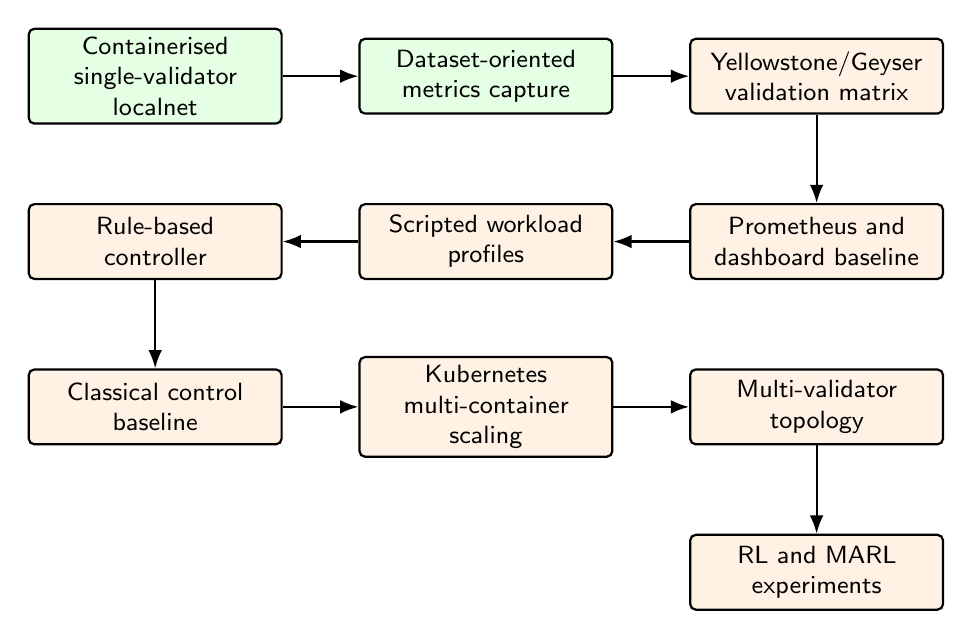
\begin{tikzpicture}[x=1cm,y=1cm]
\node[ddone] (r1) at (0,0) {Containerised\\single-validator localnet};
\node[ddone] (r2) at (4.2,0) {Dataset-oriented\\metrics capture};
\node[dplanned] (r3) at (8.4,0) {Yellowstone/Geyser\\validation matrix};
\node[dplanned] (r4) at (8.4,-2.1) {Prometheus and\\dashboard baseline};
\node[dplanned] (r5) at (4.2,-2.1) {Scripted workload\\profiles};
\node[dplanned] (r6) at (0,-2.1) {Rule-based\\controller};
\node[dplanned] (r7) at (0,-4.2) {Classical control\\baseline};
\node[dplanned] (r8) at (4.2,-4.2) {Kubernetes\\multi-container scaling};
\node[dplanned] (r9) at (8.4,-4.2) {Multi-validator\\topology};
\node[dplanned] (r10) at (8.4,-6.3) {RL and MARL\\experiments};

\draw[darrow] (r1.east) -- (r2.west);
\draw[darrow] (r2.east) -- (r3.west);
\draw[darrow] (r3.south) -- (r4.north);
\draw[darrow] (r4.west) -- (r5.east);
\draw[darrow] (r5.west) -- (r6.east);
\draw[darrow] (r6.south) -- (r7.north);
\draw[darrow] (r7.east) -- (r8.west);
\draw[darrow] (r8.east) -- (r9.west);
\draw[darrow] (r9.south) -- (r10.north);
\end{tikzpicture}
\caption{Suggested roadmap from the present Solana localnet to adaptive and multi-agent experiments. Status labels should be verified before article submission.}
\label{fig:roadmap}
\end{figure}

\subsection{Why not start directly with MARL}
\label{subsec:why-not-marl}

Multi-agent reinforcement learning is attractive because distributed systems naturally involve multiple interacting components and partially local decisions. However, MARL introduces evaluation risks. Rewards may encode the wrong behaviour. Agents may overfit to a narrow synthetic environment. Training may produce unstable policies. Comparative baselines may be weak. For these reasons, MARL should appear in the article as a long-term research direction supported by the testbed, not as an immediate result.

A staged approach is stronger:

\begin{enumerate}
  \item Build reproducible open-loop experiments.
  \item Publish datasets with complete metadata.
  \item Implement deterministic workload profiles.
  \item Add rule-based controllers and simple safety constraints.
  \item Compare against classical feedback or model-predictive baselines.
  \item Only then evaluate RL or MARL policies.
\end{enumerate}

\section{Discussion}
\label{sec:discussion}

The main methodological benefit of the proposed approach is that it treats benchmarking as a research infrastructure problem. A headline throughput result may be useful, but it is not enough to support reproducible science. A control-oriented testbed must expose what was run, where it was run, how it was measured, and how the measurements can be used for later decision-making.

The Solana case study also shows why observability is not a secondary concern. In a high-performance blockchain environment, the difference between external RPC observations and validator-side event streams can be scientifically meaningful. Geyser and Yellowstone gRPC provide a natural path for studying this difference, because they expose validator-side event flow to external consumers \cite{anza2026geyser,rpcpool2026yellowstone}. The monitor component can then transform these events into Prometheus-compatible metrics and dataset records.

At the same time, the approach has limits. A single-host localnet cannot reproduce public-network dynamics such as adversarial network delay, heterogeneous validators, stake distribution, mainnet transaction composition, or validator-client diversity. It should therefore be interpreted as a controlled laboratory environment. Its value is strongest in early-stage methodology development, instrumentation testing, workload design, and reproducibility studies.

\section{Threats to validity}
\label{sec:validity}

\begin{table}[H]
\centering
\caption{Threats to validity and mitigation strategies}
\label{tab:validity}
\begin{tabularx}{\textwidth}{L{3.2cm}Y Y}
\toprule
\textbf{Threat} & \textbf{Risk} & \textbf{Mitigation} \\
\midrule
Localnet realism & A private single-validator network may not represent public Solana behaviour. & Frame claims as testbed methodology, not mainnet performance. \\
Synthetic workload bias & Artificial transaction mixes may miss real application patterns. & Define multiple workload profiles and document assumptions. \\
Host dependence & Results may depend strongly on CPU, memory, disk, and container engine. & Include hostname and hardware metadata in every dataset. \\
Observability overhead & Geyser, monitor, and metrics exporters may affect the system being measured. & Run with and without observability components where possible. \\
Clock alignment & Event timing may be distorted by clock differences or timestamp placement. & Record timestamp sources and use consistent time standards. \\
Version drift & Solana, Agave, Yellowstone, and container images may change over time. & Pin versions and record image digests. \\
Controller overclaiming & Future RL or MARL claims may exceed what the testbed validates. & Use staged baselines and clearly distinguish implemented work from roadmap. \\
Publication mismatch & Repository state may diverge from article claims. & Synchronise README, release notes, DOI records, and article text before submission. \\
\bottomrule
\end{tabularx}
\end{table}

\section{Conclusion}
\label{sec:conclusion}

This paper argued that synthetic benchmarking in distributed systems is evolving from a tool for measuring performance towards a methodology for building reproducible, observable, and eventually controllable experimental environments. The proposed framing does not discard traditional performance metrics. Instead, it places them inside a wider research loop that includes workload generation, telemetry, dataset publication, and control interfaces.

The containerised Solana localnet case study illustrates this transition. A validator-centred private network, augmented with Yellowstone/Geyser observability, monitor services, Prometheus-compatible metrics, and DOI-backed research \artifacts{}, can serve as a practical foundation for studying high-performance blockchain behaviour under controlled conditions. The preliminary empirical pilot strengthens the paper by showing that the data-collection workflow can distinguish baseline execution from controlled transaction-load profiles while preserving metadata, RPC counters, and workload-side transaction evidence. All included pilot samples returned healthy validator status, and transaction-load profiles produced transaction-count deltas consistent with the workload-side successful transfer counts.

The pilot should not be read as a final performance study. It is a single-host validation of the measurement pipeline and article methodology. The next repository step is to integrate the article and derived pilot summaries through a narrow GitHub commit, using the operational workflow specified in this manuscript. The next empirical step is to extend the matrix with paired observability-overhead runs, Geyser/Yellowstone stream-latency measurements, and cross-host repetitions. Only after these baselines are stable should the work move towards rule-based control, control-theoretic baselines, and later multi-agent reinforcement learning experiments.

\appendix

\section{Proposed figure list for the final article}
\label{app:figure-list}

\begin{longtable}{L{1.2cm}L{4.0cm}L{9.0cm}}
\caption{Planned visual material for the article}\label{tab:figure-list}\\
\toprule
\textbf{No.} & \textbf{Figure} & \textbf{Purpose} \\
\midrule
\endfirsthead
\toprule
\textbf{No.} & \textbf{Figure} & \textbf{Purpose} \\
\midrule
\endhead
1 & Conceptual progression & Show transition from benchmark to testbed, dataset, and controller. \\
2 & Benchmark evolution timeline & Summarise historical development of benchmark goals. \\
3 & Open-loop versus closed-loop & Explain the control-oriented framing. \\
4 & Control maturity path & Present staged progression towards MARL. \\
5 & Requirement layers & Connect scientific and engineering layers. \\
6 & Solana testbed architecture & Show validator, workload, monitor, Geyser, and datasets. \\
7 & Geyser observability path & Explain validator-side streaming. \\
8 & Experiment lifecycle & Show repeatable benchmark procedure. \\
9 & Time-series metric illustration & Demonstrate multi-metric analysis style. \\
10 & Artefact publication pipeline & Link code, release, DOI, datasets, and paper evidence. \\
11 & Repository integration map & Show how article source, documentation, datasets, PDF, and DOI records are connected. \\
12 & Research roadmap & Show future development stages. \\
\bottomrule
\end{longtable}

\section{Proposed table list for the final article}
\label{app:table-list}

\begin{longtable}{L{1.2cm}L{4.0cm}L{9.0cm}}
\caption{Planned tables for the article}\label{tab:table-list}\\
\toprule
\textbf{No.} & \textbf{Table} & \textbf{Purpose} \\
\midrule
\endfirsthead
\toprule
\textbf{No.} & \textbf{Table} & \textbf{Purpose} \\
\midrule
\endhead
1 & Research questions & State the methodological questions guiding the article. \\
2 & Terminology & Prevent confusion between benchmark, testbed, workload, dataset, and controller. \\
3 & Benchmark objectives & Compare historical phases and limitations. \\
4 & Requirements & Define design requirements for control-oriented benchmarking. \\
5 & Implementation boundary & Separate completed artefacts, target architecture, and future work. \\
6 & Component responsibilities & Map Solana components to research roles. \\
7 & Experimental matrix & Specify variables, measured signals, and required artefacts for future empirical work. \\
8 & Experiment classes & Define the empirical validation classes. \\
9 & Metric taxonomy & Organise metrics for analysis and control. \\
10 & Dataset metadata & Standardise reproducibility fields. \\
11 & Evidence plan & Connect future empirical claims to required datasets and metrics. \\
12 & Data-readiness triggers & Specify when empirical datasets become necessary. \\
13 & Artefact classes & Define publication outputs. \\
14 & Repository layout & Define where the article, documentation, scripts, and future datasets should live. \\
15 & Threats to validity & Support rigorous discussion. \\
\bottomrule
\end{longtable}


\section{Repository integration checklist}
\label{app:repository-integration-checklist}

Before committing the article to the repository, use the following checklist.

\begin{itemize}
  \item Create a dedicated article directory such as \path{paper/synthetic-benchmarks-solana/}.
  \item Copy \texttt{main.tex}, \texttt{references.bib}, \texttt{main.bbl}, \texttt{main.pdf}, and \texttt{README.md} into the article directory.
  \item Add a repository-facing status document under \path{docs/research-program/}.
  \item State clearly that the current manuscript is methodological and does not yet contain empirical Solana performance results.
  \item Add build instructions that work with BibTeX and with the included \texttt{main.bbl} fallback.
  \item Do not place raw datasets inside the article directory.
  \item Commit dataset templates separately from empirical datasets.
  \item Check that README, article, release notes, and Zenodo records use the same terminology for completed work and future work.
\end{itemize}

A conservative copy plan is:

\begin{verbatim}
paper/synthetic-benchmarks-solana/
  main.tex
  references.bib
  main.bbl
  main.pdf
  README.md
  README_BUILD.md

docs/research-program/
  synthetic-benchmarks-solana-article.md
  article-status.md

prompts/codex/
  21_github_integration_workflow_v1_1.md

scripts/
  build_synthetic_benchmarks_article.sh
  integrate_synthetic_benchmark_article_v1_1.sh
  check_synthetic_benchmark_article_integration.sh
\end{verbatim}

\section{Local GitHub integration command sheet}
\label{app:github-command-sheet}

This appendix provides a compact command sheet for integrating the article into a local repository clone. It is intended for repository maintenance rather than for article review.

\begin{verbatim}
# Local assumptions:
# - repository clone: ~/project/solana-containerised-testbed
# - extracted v1.1 package: ~/Downloads/solana_benchmark_article_v1_1

cd ~/project/solana-containerised-testbed

git branch --show-current
git status --short

PKG=~/Downloads/solana_benchmark_article_v1_1/repository-integration

bash "$PKG/scripts/integrate_synthetic_benchmark_article_v1_1.sh" \
  "$PKG" \
  "$(pwd)"

bash scripts/build_synthetic_benchmarks_article.sh \
  paper/synthetic-benchmarks-solana

bash scripts/check_synthetic_benchmark_article_integration.sh

git status --short
git diff --stat

git add \
  paper/synthetic-benchmarks-solana \
  docs/research-program/synthetic-benchmarks-solana-article.md \
  docs/research-program/article-status.md \
  prompts/codex/21_github_integration_workflow_v1_1.md \
  scripts/build_synthetic_benchmarks_article.sh \
  scripts/integrate_synthetic_benchmark_article_v1_1.sh \
  scripts/check_synthetic_benchmark_article_integration.sh

git commit -m "docs: add synthetic benchmarking article integration workflow"
git push
\end{verbatim}

A slightly more explicit commit body is:

\begin{verbatim}
Add article source, generated review PDF, repository-facing status pages,
local integration helpers, and a Codex prompt for the synthetic benchmarking
article. The draft remains methodological and does not introduce empirical
Solana performance, overhead, stream-latency, reproducibility, or controller
claims.
\end{verbatim}

\section{Data handover checklist for an empirical revision}
\label{app:data-handover}

When the manuscript moves from the present methodological version to an empirical version, the first dataset handover should be small, structured, and easy to audit. A recommended first archive should contain one directory per run and should avoid mixing raw data, derived data, and figures.

\begin{table}[H]
\centering
\caption{Recommended first data handover package}
\label{tab:first-data-handover}
\begin{tabularx}{\textwidth}{L{3.2cm}Y Y}
\toprule
\textbf{Package element} & \textbf{Minimum content} & \textbf{Purpose} \\
\midrule
Baseline runs & Three clean validator/localnet boot runs. & Establish reproducible startup and health-check behaviour. \\
Transaction-load runs & Two profiles, preferably low and medium load. & Provide the first latency, success-rate, and resource-use evidence. \\
Observability pair & One matched workload run with observability off and on. & Estimate the monitoring and Geyser/Yellowstone overhead. \\
Run metadata & One \texttt{metadata.json} per run. & Link every measurement to version, host, workload, and configuration. \\
Host metadata & One \texttt{host.json} per host. & Explain cross-host and hardware-dependent differences. \\
Raw metrics & CSV or JSONL files with timestamps. & Preserve primary evidence without manual editing. \\
Logs & Validator, workload, and monitor logs. & Support debugging and interpretation. \\
Checksums & One \texttt{checksums.sha256} per run bundle. & Protect against accidental file changes after publication. \\
\bottomrule
\end{tabularx}
\end{table}

The preferred upload format is a single ZIP archive. The archive should be named with a project prefix and dataset version, for example \texttt{solana-testbed-datasets-v0.1.zip}. If the first archive is large, a smaller pilot archive with one baseline run and one transaction-load run should be reviewed first.

\section{Dataset metadata templates}
\label{app:metadata-templates}

This appendix defines practical metadata templates for future dataset-producing runs. The exact field names may evolve with the repository, but every empirical version of the article should preserve the same principle: a dataset is incomplete unless it records the run identity, host identity, source identity, container identity, workload identity, observability settings, and output checksums.

\subsection{Minimal run metadata JSON}
\label{app:minimal-run-json}

\begin{verbatim}
{
  "run_id": "20260515T121500Z_hpz440_txload-low_300s",
  "timestamp_utc": "2026-05-15T12:15:00Z",
  "hostname": "hpz440",
  "operator": "okhoshaba",
  "project": "solana-containerised-testbed",
  "git_repository": "https://github.com/okhoshaba/solana-containerised-testbed",
  "git_branch": "main",
  "git_commit": "a1b2c3d",
  "git_dirty": false,
  "compose_file": "compose.yellowstone.yaml",
  "container_engine": "podman",
  "container_engine_version": "REPLACE_WITH_VERSION",
  "solana_version": "1.18.25",
  "agave_or_validator_image": "REPLACE_WITH_IMAGE_TAG",
  "image_digest": "sha256:REPLACE_WITH_DIGEST",
  "workload_profile": "txload-low",
  "duration_seconds": 300,
  "random_seed": 12345,
  "geyser_enabled": true,
  "yellowstone_enabled": true,
  "prometheus_enabled": true,
  "prometheus_scrape_interval_seconds": 5,
  "ledger_reset": true,
  "notes": "Short free-text note about the run."
}
\end{verbatim}

\subsection{Host metadata JSON}
\label{app:host-json}

\begin{verbatim}
{
  "hostname": "hpz440",
  "os": "Ubuntu 24.04 LTS",
  "kernel": "REPLACE_WITH_KERNEL",
  "cpu_model": "REPLACE_WITH_CPU_MODEL",
  "cpu_cores": 8,
  "memory_gb": 32,
  "disk_type": "SSD",
  "container_engine": "podman",
  "container_engine_version": "REPLACE_WITH_VERSION",
  "clock_sync": "REPLACE_WITH_NTP_OR_CHRONY_STATUS"
}
\end{verbatim}

\subsection{Workload profile YAML}
\label{app:workload-yaml}

\begin{verbatim}
profile_name: txload-low
profile_version: 1
purpose: Conservative transaction-load validation profile.
duration_seconds: 300
warmup_seconds: 30
cooldown_seconds: 30
target_transaction_rate_per_second: 5
burst_mode: false
request_mix:
  transfer_transactions: 1.0
random_seed: 12345
payer_account: default
recipient_account_policy: generated
expected_outputs:
  - metrics_csv
  - workload_log
  - metadata_json
  - summary_json
\end{verbatim}

\subsection{Recommended dataset bundle}
\label{app:dataset-bundle}

A complete run bundle should use a stable directory name based on timestamp, hostname, profile, duration, and short commit hash. A minimal bundle should contain:

\begin{verbatim}
20260515T121500Z_hpz440_txload-low_300s_a1b2c3d/
  metadata.json
  host.json
  workload-profile.yaml
  container-images.txt
  compose-file-copy.yaml
  raw-metrics.csv
  workload.log
  validator-health.jsonl
  summary.json
  checksums.sha256
\end{verbatim}

The file \texttt{checksums.sha256} should be generated after the run and before publication. Derived datasets and article figures should not overwrite raw files; they should be stored separately or generated by scripts from immutable raw inputs.

\section{Draft checklist before submission}
\label{app:checklist}

\begin{itemize}
  \item Replace placeholder author metadata.
  \item Verify the current repository state against every claim in the paper.
  \item Verify that the article source is stored in a dedicated repository directory with build instructions.
  \item Verify that repository-facing documentation links to the article without duplicating the full manuscript.
  \item Check that README, release notes, Zenodo records, and article claims use the same implementation status.
  \item Add exact Solana, Agave, Yellowstone, Docker/Podman, and Prometheus versions.
  \item Record container image tags and image digests for every experiment.
  \item Add profile files for boot-baseline, txload-low, txload-step, rpc-pressure, obs-off, obs-on, geyser-latency, resource-limit, and cross-host runs.
  \item Request empirical datasets only when the manuscript introduces quantitative performance, overhead, stream-latency, reproducibility, or controller claims.
  \item Replace the schematic time-series figure with measured results.
  \item Add measured observability-overhead results from paired runs.
  \item Add hostname-aware dataset examples from at least two machines if available.
  \item Publish raw data, derived data, plotting scripts, metadata JSON files, workload profiles, and checksums.
  \item Confirm Zenodo DOI metadata and cite exact versions.
  \item Ensure all future work is clearly separated from completed implementation.
  \item Review whether any claim implies mainnet behaviour; if so, either add evidence or narrow the claim.
\end{itemize}

\bibliographystyle{plainnat}
\bibliography{references}

\end{document}
